\section{Stations-Topologie}%\addcontentsline{toc}{section}{Topologische Folgerungen}
\label{sec:topologie}
\fancyhead[RO]{Stations-Topologie}
% \fancyhead[LO]{}

\paragraph{Notwendigkeit}

Nicht alle kanonischen Aussagen über die \ceva{ringe} lassen sich befriedigend anhand der konventionellen Darstellungsweise der \ring{ringe} als konzentrische Kreise (\cref{fig:ringconvention}) demonstrieren. 

So stellt sich die Frage: welche nicht-euklidische Topologie
\begin{enumerate}
    \item erklärt die Berührung von Innen (\ceva{core}) und Außen (\ceva{clamp})
    \item erklärt die Sonderstellung des mittleren Rings \ceva{creactive}
    \item kann durch Abbildung in die konventionelle Ansicht überführt werden?
\end{enumerate}
Dieser Frage gehen wir im Folgenden nach. 

\paragraph{Verflachung}
Die aktuelle Form ist Folge des den Absturzes der Raumstation, und vermutlich ist die gewissermaßen "`flache"' Struktur, die wir bei den bisherigen Rekonstruktionsphasen ausgemacht haben, eine zweidimensionale Projektion der eigentlich mehrdimensionalen Raumstation (\cref{eq:grundgleichung}). 

Diese Frage stellt sich: welche Topologie hatten die \ring{ringe}, welche Topologie hatte die Station vor dem Absturz, und welche strebt sie damit an? Wir gehen im Folgenden nicht auf die Möglichen $m$- oder $n$-dimensionalen Räume ein, sondern beschränken uns der Einfachheit halber auf zweidimensionale Mannigfaltigkeiten.

\begin{figure}[ht!]
    \centering
    \begin{subfigure}{0.4\textwidth}
        \centering
        \resizebox{\textwidth}{!}{
        \documentclass{standalone}
\usepackage{tikz}
\usetikzlibrary{decorations, decorations.text}
\usepackage{calc}
\usepackage{xcolor}
\usepackage{fontspec}
\newcommand{\ceva}[1]{~{\fontspec{[ceva-c2.ttf]}#1}}
\definecolor{eins}{HTML}{e7e7e8}   %% Ring 1 "core"     - weiß - Mittelpunkt, Ring um Mittelpunkt
\definecolor{zwei}{HTML}{ed1c24}   %% Ring 2 "com"      - rot -  "Fenster" innen
\definecolor{drei}{HTML}{fbad18}   %% Ring 3  "culture" - orange - fünf Module, quasi invertiert
\definecolor{vier}{HTML}{74c043}   %% Ring 4  "creactiv" - grün -  vier Module
\definecolor{fuenf}{HTML}{0089d0}  %% Ring 5 "cience"  - cyan (blau) - drei Module mit "Strich"
\definecolor{sechs}{HTML}{11357e}  %% Ring 6 "carbon" -  indigo - viele "Fenster" außen
\definecolor{sieben}{HTML}{000000} %% Ring 7 "clamp" -  schwarz, c-förmig
\definecolor{cbase}{HTML}{222222}  %% Körper der Raumstation    
\begin{document}
%% c-base logo nachgebaut von penta.
%% alles nur geschätze Winkel und Abstände :/
%% um den code zu verstehen, einfach mal einzelne Teile auskommentieren und wieder einkommentieren (ctrl-#) und dann mal \draw[white] durch \draw[red] ersetzen, dann sieht man, was was ist.
%% viel Spaß damit.
\tikzset{
  pics/carc/.style args={#1:#2:#3:#4}{
    code={
      \draw[postaction={decorate, decoration={text along path, raise=-2pt, text align={align=center}, text={\ceva{#4}}, reverse path}}] (#1:#3) arc(#1:#2:#3);
    }
  }
}%
    \begin{tikzpicture}
        \draw[gray, line width=50pt] (0:0) circle (3);
        \foreach [count=\i] \ring/\color in
            {core/eins,com/zwei,culture/drei,creactiv/vier,cience/fuenf,carbon/sechs,clamp/sieben}
            {%
                \draw[color=\color!50,line width=45pt] (0:0) pic{carc=\i*51.418-25:\i*51.418+25:3:\ring};
            }%
    \end{tikzpicture}
\end{document}
    
        }
    \end{subfigure}
    \hspace{2ex}
    \begin{subfigure}{0.4\textwidth}
        \centering
       \resizebox{\textwidth}{!}{
        \documentclass{standalone}
\usepackage{tikz}
\usetikzlibrary{decorations, decorations.text}
\usepackage{calc}
\usepackage{xcolor}
\usepackage{fontspec}
\newcommand{\cevapic}[1]{~{\fontspec{[ceva-c2.ttf]}#1}}
\definecolor{eins}{HTML}{e7e7e8}   %% Ring 1 "core"     - weiß - Mittelpunkt, Ring um Mittelpunkt
\definecolor{zwei}{HTML}{ed1c24}   %% Ring 2 "com"      - rot -  "Fenster" innen
\definecolor{drei}{HTML}{fbad18}   %% Ring 3  "culture" - orange - fünf Module, quasi invertiert
\definecolor{vier}{HTML}{74c043}   %% Ring 4  "creactiv" - grün -  vier Module
\definecolor{fuenf}{HTML}{0089d0}  %% Ring 5 "cience"  - cyan (blau) - drei Module mit "Strich"
\definecolor{sechs}{HTML}{11357e}  %% Ring 6 "carbon" -  indigo - viele "Fenster" außen
\definecolor{sieben}{HTML}{000000} %% Ring 7 "clamp" -  schwarz, c-förmig
\definecolor{cbase}{HTML}{222222}  %% Körper der Raumstation    
\begin{document}
 
% \tikzset{
%   pics/carc/.style args={#1:#2:#3:#4}{
%     code={
%       \draw[postaction={decorate, decoration={text along path, raise=-2pt, text align={align=center}, text={\cevapic{#4}}, reverse path}}] (#1:#3) arc(#1:#2:#3);
%     }
%   }
% }%
    \begin{tikzpicture}[scale=0.4]
        % \draw[gray, line width=50pt] (0:0) circle (3);
        \foreach [count=\i] \ring/\color in
            {clamp/sieben,carbon/sechs,cience/fuenf,creactiv/vier,culture/drei,com/zwei,core/white}
            {%
                \draw[line width=12pt,draw=black] (\i*51.4286:5) circle (2.5);
                \draw[line width=10pt,draw=\color] (\i*51.4286:5) circle (2.5);
                \node [fill=\color!40,rounded corners,draw] at (\i*51.4286:5){\cevapic{\ring}};
                % \draw[color=\color!50,line width=45pt] (0:0) pic{carc=\i*51.418-25:\i*51.418+25:3:\ring};
            }%
            % \draw[color=white,line width=122] (0:0) pic{carc=-21:21:2.5:};
    \end{tikzpicture}
\end{document}

        }
    \end{subfigure}
    
    \caption{Ringförmige Anordnungen der \ring{ringe}}
    \label{fig:ringring}
\end{figure}

\paragraph{Ringförmige Anordnung der Ringe}
Wir haben gesehen, dass sich \ceva{clamp} und \ceva{core} berühren bzw. über eine Einstein-Rosen-Brücke verbunden sind. Daraus folgern wir eine (ursprünglich, zukünftig) \emph{ringförmige Anordnung der Ringe;} solche Ordnungen sind beispielhaft abgebildet in \cref{fig:ringring}. Jeder Ring tangiert unmittelbar jeden benachbarten Ring.



\paragraph{Rotationstorus}
Eine \emph{ringförmige Anordnung von Ringen }ist topologisch darstellbar als Fläche, die entsteht, wenn ein Kreis um einen Kreis (also quasi ein \ring{ring} um einen \ring{ring}) rotiert. Diese Figur ist der \emph{Rotationstorus}.

\cref{fig:torusweiss}  zeigt ein toroidales Polyeder mit $14\times 14$ Flächen als Annäherung an den Rotationstorus. Eine solche Geometrie ist unter anderem für den \cevain{coremechanism} belegt (\cite[S.32f.]{cbasebook}).

\begin{figure}[ht!]
    \centering
    \documentclass{standalone}
\usepackage{xcolor}
\usepackage[svgnames]{pstricks}
\usepackage{pst-solides3d}
\definecolor{eins}{HTML}{e7e7e8}   %% Ring 1 "core"     - weiß - Mittelpunkt, Ring um Mittelpunkt
\definecolor{zwei}{HTML}{ed1c24}   %% Ring 2 "com"      - rot -  "Fenster" innen
\definecolor{drei}{HTML}{fbad18}   %% Ring 3  "culture" - orange - fünf Module, quasi invertiert
\definecolor{vier}{HTML}{74c043}   %% Ring 4  "creactiv" - grün -  vier Module
\definecolor{fuenf}{HTML}{0089d0}  %% Ring 5 "cience"  - cyan (blau) - drei Module mit "Strich"
\definecolor{sechs}{HTML}{11357e}  %% Ring 6 "carbon" -  indigo - viele "Fenster" außen
\definecolor{sieben}{HTML}{000000} %% Ring 7 "clamp" -  schwarz, c-förmig
\definecolor{cbase}{HTML}{222222}  %% Körper der Raumstation    
\begin{document}

%% https://ftp.tu-chemnitz.de/pub/tex/graphics/pstricks/contrib/pst-solides3d/doc/pst-solides3d-doc.pdf

\begin{pspicture}(-4,-4)(4,4)
    \psset{Decran=20,viewpoint=5 11 25}
    \pstVerb{/iface 0 store}%
    \psSolid[
        r1=3,r0=2,
        object=tore,
        ngrid=14 14,
        RotY=30]
\end{pspicture}


\end{document}
    \caption{Toroidales Polyeder imt $14\times 14$ Flächen} 
    % Es hat 14  Meridiane und 14 Parallelkreise (angenähert)
    \label{fig:torusweiss}
\end{figure}

Nun stellt sich die Frage, wie die \ring{ringe} auf so einem Torus angeordnet waren bzw. sein werden bzw. sollen. 
Grundsätzlich sind die \ring{ringe} Kreisscharen. 

\parbox{\textwidth}{
    Es gibt genau drei unterscheidbare Gruppen von Kreisscharen auf einem Torus: 
    \begin{enumerate}
        \item Parallelkreise (poloidal)
        \item Merididiane (toroidal) und 
        \item Villarceau-Kreise.
    \end{enumerate}
    }
Diese drei Möglichkeiten betrachten wir im Folgenden etwas näher.

\paragraph{Parallelkreise} entstehen durch poloidale Schnitte eines wie z.B. in \cref{fig:torus-parallele} abgebildeten Torus. Eine solche Anordnung der \ring{ringe} ist denkbar, aber wenig plausibel, da die einzelnen Ringe dann eher Schreiben wären. Auch ist nicht zu erkennen, wie es beim Absturz der Station dann zu einer konzentrischen Anordnung gekommen sein sollte. 

\begin{figure}[ht!]
    \centering
    \documentclass{standalone}
\usepackage{xcolor}
\usepackage[svgnames]{pstricks}
\usepackage{pst-solides3d}
\definecolor{eins}{HTML}{e7e7e8}   %% Ring 1 "core"     - weiß - Mittelpunkt, Ring um Mittelpunkt
\definecolor{zwei}{HTML}{ed1c24}   %% Ring 2 "com"      - rot -  "Fenster" innen
\definecolor{drei}{HTML}{fbad18}   %% Ring 3  "culture" - orange - fünf Module, quasi invertiert
\definecolor{vier}{HTML}{74c043}   %% Ring 4  "creactiv" - grün -  vier Module
\definecolor{fuenf}{HTML}{0089d0}  %% Ring 5 "cience"  - cyan (blau) - drei Module mit "Strich"
\definecolor{sechs}{HTML}{11357e}  %% Ring 6 "carbon" -  indigo - viele "Fenster" außen
\definecolor{sieben}{HTML}{000000} %% Ring 7 "clamp" -  schwarz, c-förmig
\definecolor{cbase}{HTML}{222222}  %% Körper der Raumstation    
\begin{document}

%% https://ftp.tu-chemnitz.de/pub/tex/graphics/pstricks/contrib/pst-solides3d/doc/pst-solides3d-doc.pdf

\begin{pspicture}(-4,-4)(4,4)
    \psset{Decran=20,viewpoint=5 11 25}
    \pstVerb{/iface 0 store}%
    \psSolid[
        hue = 0 1,
        % fcol=48 {iface (green)
        % iface 1 add (orange)
        % iface 2 add (orange)
        % iface 3 add (red) 
        % iface 4 add (red) 
        % iface 5 add (white) 
        % iface 6 add (white) 
        % iface 7 add (black) 
        % iface 8 add (black) 
        % iface 9 add (blue) 
        % iface 10 add (blue) 
        % iface 11 add (blue) 
        % iface 12 add (blue) 
        % iface 13 add (blue) /iface
        % iface 14 add store} repeat,
        r1=3,r0=2,
        object=tore,
        ngrid=14 14,
        RotY=30]
\end{pspicture}


\end{document}
    \caption{Parallelkreise}
    \label{fig:torus-parallele}
\end{figure}

\paragraph{Meridiankreise} entstehen als toridale Schnitte des Rotationstorus. 
Eine Anodrnung der \ring{ringe} als Meridiankreise  zeigt \cref{fig:torus-meridiane}.  
Dabei berühren sich hier im Inneren eben \ceva{core} und \ceva{clamp}; das passt zu unserer Interpretation des Kanons von der Topologie der Station als Torus mit einem innenliegenden Wurmloch. In diesem berühren sich innen \ceva{core} und \ceva{clamp}; außen liegt \ceva{creactiv}. 

\begin{figure}[ht!]
    \centering
    % \begin{subfigure}{0.4\textwidth}
    %     \documentclass{standalone}
\usepackage{xcolor}
\usepackage[svgnames]{pstricks}
\usepackage{pst-solides3d}
\definecolor{eins}{HTML}{e7e7e8}   %% Ring 1 "core"     - weiß - Mittelpunkt, Ring um Mittelpunkt
\definecolor{zwei}{HTML}{ed1c24}   %% Ring 2 "com"      - rot -  "Fenster" innen
\definecolor{drei}{HTML}{fbad18}   %% Ring 3  "culture" - orange - fünf Module, quasi invertiert
\definecolor{vier}{HTML}{74c043}   %% Ring 4  "creactiv" - grün -  vier Module
\definecolor{fuenf}{HTML}{0089d0}  %% Ring 5 "cience"  - cyan (blau) - drei Module mit "Strich"
\definecolor{sechs}{HTML}{11357e}  %% Ring 6 "carbon" -  indigo - viele "Fenster" außen
\definecolor{sieben}{HTML}{000000} %% Ring 7 "clamp" -  schwarz, c-förmig
\definecolor{cbase}{HTML}{222222}  %% Körper der Raumstation    
\begin{document}

%% https://ftp.tu-chemnitz.de/pub/tex/graphics/pstricks/contrib/pst-solides3d/doc/pst-solides3d-doc.pdf

\begin{pspicture}(-4,-4)(4,4)
    \psset{Decran=20,viewpoint=5 11 25}
    \pstVerb{/iface 0 store}%
    \psSolid[
        fcol=48 {iface (green)
        iface 1 add (orange)
        iface 2 add (orange)
        iface 3 add (red) 
        iface 4 add (red) 
        iface 5 add (white) 
        iface 6 add (white) 
        iface 7 add (black) 
        iface 8 add (black) 
        iface 9 add (blue) 
        iface 10 add (blue) 
        iface 11 add (blue) 
        iface 12 add (blue) 
        iface 13 add (blue) /iface
        iface 14 add store} repeat,
        r1=3,r0=2,
        object=tore,
        ngrid=14 14,
        RotY=30]
\end{pspicture}


\end{document}
    % \end{subfigure}
    % \begin{subfigure}{0.4\textwidth}
        \documentclass{standalone}
\usepackage{xcolor}
\usepackage[svgnames]{pstricks}
\usepackage{pst-solides3d}
\definecolor{eins}{HTML}{e7e7e8}   %% Ring 1 "core"     - weiß - Mittelpunkt, Ring um Mittelpunkt
\definecolor{zwei}{HTML}{ed1c24}   %% Ring 2 "com"      - rot -  "Fenster" innen
\definecolor{drei}{HTML}{fbad18}   %% Ring 3  "culture" - orange - fünf Module, quasi invertiert
\definecolor{vier}{HTML}{74c043}   %% Ring 4  "creactiv" - grün -  vier Module
\definecolor{fuenf}{HTML}{0089d0}  %% Ring 5 "cience"  - cyan (blau) - drei Module mit "Strich"
\definecolor{sechs}{HTML}{11357e}  %% Ring 6 "carbon" -  indigo - viele "Fenster" außen
\definecolor{sieben}{HTML}{000000} %% Ring 7 "clamp" -  schwarz, c-förmig
\definecolor{cbase}{HTML}{222222}  %% Körper der Raumstation    
\begin{document}

%% https://ftp.tu-chemnitz.de/pub/tex/graphics/pstricks/contrib/pst-solides3d/doc/pst-solides3d-doc.pdf

\begin{pspicture}(-4,-4)(4,4)
    \psset{Decran=20,viewpoint=5 11 25}
    \pstVerb{/iface 0 store}%
    \psSolid[
        fcol=48 {iface (green)
        iface 1 add (orange)
        iface 2 add (red) 
        iface 3 add (white) 
        iface 4 add (black) 
        iface 5 add (blue) 
        iface 6 add (blue) /iface
        iface 7 add store} repeat,
        r1=3,r0=2,
        object=tore,
        ngrid=7 14,
        RotY=30]
\end{pspicture}


\end{document}
    % \end{subfigure}
    \caption{Die \ring{ringe} als Meridiankreise auf dem Torus}
    \label{fig:torus-meridiane}
\end{figure}

Eine solche Anordnung erscheint dem archälogischen Befund recht gut zu entsprechen. Sie kann aber ihrerseits Produkt einer vorhergegangenen Translation aus einer komplexeren Struktur sein.

Da der äußerere Äquator (Meridian) des Torsus \ceva{creactive} enspricht, bedeutet eine Ausweitung der \ceva{creactivität} ein Anschwellen dieses Torus und somit Wachstum der Station; bildlich entspräche das in etwa der Inflation eines Rettungsrings. Dabei ist zu beachten, dass eine Vergrößerung des rotierenden Kreises ohne gleichzeitige Ausweitung des Rototaionsradius im Torus zu einem Verschwinden des innenliegenden Loches führen könnte. Dann wäre die Station gewissermaßen an ihrer eigenen \ceva{creactivität} erstickt.

Unsere Darstellung in \cref{fig:torus-meridiane} zeigt die \ring{ringe} als Flächen. Tatsächlich sind sie natürlich selbst von höherer Diemension, also ihrerseits Tori. Es sollte sich wirklich um eine Schar von Tori, gewissermaßen um ein Bündel von Ringen, handeln.

\paragraph{Villarcreau-Kreise}
Betrachten wir nun die vielleicht interessanteste mögliche Anordnung von Kreisscharen auf einem Torso. Villarceau-Kreise  entstehen topologisch (paarweise) durch den Schnitt einer doppelberührenden Ebene mit dem Torso (\cref{fig:villarceaukreise}).

\begin{figure}[ht!]
    \centering
    \includesvg{Torus-vill-point.svg}
    \caption{Villarceau-Kreise} Quelle:  \cite{villarceauag2gaeh}
    \label{fig:villarceaukreise}
\end{figure}

Es lässt sich also eine Schar von Kreisen auf einem Torus finden, die sich nicht schneiden, die perfekt kreisförmig und die untereinander kongruent sind. \cref{fig:villarceautorous} zeigt eine Annäherung, indem hier ein Torus mit $21\times 21$ Flächen belegt wurde.

\begin{figure}[ht!] 
    \centering
            \documentclass{standalone}
\usepackage{xcolor}
\usepackage[svgnames]{pstricks}
\usepackage{pst-solides3d}
\definecolor{eins}{HTML}{e7e7e8}   %% Ring 1 "core"     - weiß - Mittelpunkt, Ring um Mittelpunkt
\definecolor{zwei}{HTML}{ed1c24}   %% Ring 2 "com"      - rot -  "Fenster" innen
\definecolor{drei}{HTML}{fbad18}   %% Ring 3  "culture" - orange - fünf Module, quasi invertiert
\definecolor{vier}{HTML}{74c043}   %% Ring 4  "creactiv" - grün -  vier Module
\definecolor{fuenf}{HTML}{0089d0}  %% Ring 5 "cience"  - cyan (blau) - drei Module mit "Strich"
\definecolor{sechs}{HTML}{11357e}  %% Ring 6 "carbon" -  indigo - viele "Fenster" außen
\definecolor{sieben}{HTML}{000000} %% Ring 7 "clamp" -  schwarz, c-förmig
\definecolor{cbase}{HTML}{222222}  %% Körper der Raumstation    
\begin{document}

%% https://ftp.tu-chemnitz.de/pub/tex/graphics/pstricks/contrib/pst-solides3d/doc/pst-solides3d-doc.pdf

\begin{pspicture}(-4,-4)(4,4)
    \psset{Decran=20,viewpoint=5 11 25}
    \pstVerb{/iface 0 store}%
    \psSolid[
        fcol=48 {iface (green)
        iface 1 add (orange)
        iface 2 add (orange)
        iface 3 add (red) 
        iface 4 add (red) 
        iface 5 add (white) 
        iface 6 add (white) 
        iface 7 add (black) 
        iface 8 add (black) 
        iface 9 add (blue) 
        iface 10 add (blue) 
        iface 11 add (SkyBlue) 
        iface 12 add (SkyBlue) 
        iface 13 add (green) /iface
        iface 14 add store} repeat,
        r1=3,r0=2,
        object=tore,
        ngrid=27 14,
        RotY=30]
\end{pspicture}

\end{document}            
    \caption{Die \ceva{Ringe} als Villarceau-Kreise} Approximation auf einem toroidalen Polyeder mit $21\times21$ Flächen
    \label{fig:villarceautorous}
\end{figure}


Dieser Theorie zufolge sind die \ring{ringe} sind auf einem Torus in Form verschlungener Bänder angeordnet. Sie winden sich um das Zentrum des Torus und zugleich um den Körper des Torus selbst. 
Es gibt keinen \ring{ring}, der einen bevorzugten Ort einnimmt. Da sie kongruent sind, sind sie flächen- und längengleich.


Wir müssen uns die Ringe nicht exakt wie abgebildet vorstellen, sondern ihrerseits eher als eigenständige Tori oder Toroide. Ähnlich wie ein Torus (2D, eine Fläche) aus Vil\-lac\-reau-Kreisen "`zusammengesetzt"' vorgestellt werden kann, kann ein Toroid (3D, ein Körper, gewissermaßen ein "`ausgefüllter"' Torus) aus Scharen von Tori "`zusammengesetzt"' bzw. approximiert werden. 
Wir können uns also die \ring{ringe} in \cref{fig:villarceautorous} als eigene Tori vorstellen.
Das setzt allerdings voraus, dass die \ring{ringe} eindeutig abgegrenzt sind gegeneinander: jeder \ring{ring} schließt sich nach einer vollen Umdrehung um die Mittelachse des Torus. 

\paragraph{Verknoteter Torus}
Lässt man die Bedingung fallen, dass jeder Ring kreisförmig und geschlossen ist, so kann man sich auch einen Torus vorstellen, bei dem jeder Kreis nach $306^o$ an den jeweils nächsten "`anschließt"', also einen "`verknoteten Torus"' bzw. \cevain{cnoten}, wie skizziert in \cref{fig:knottedtorus}.

\begin{figure}
    \centering
    \resizebox{0.5\textwidth}{!}{
        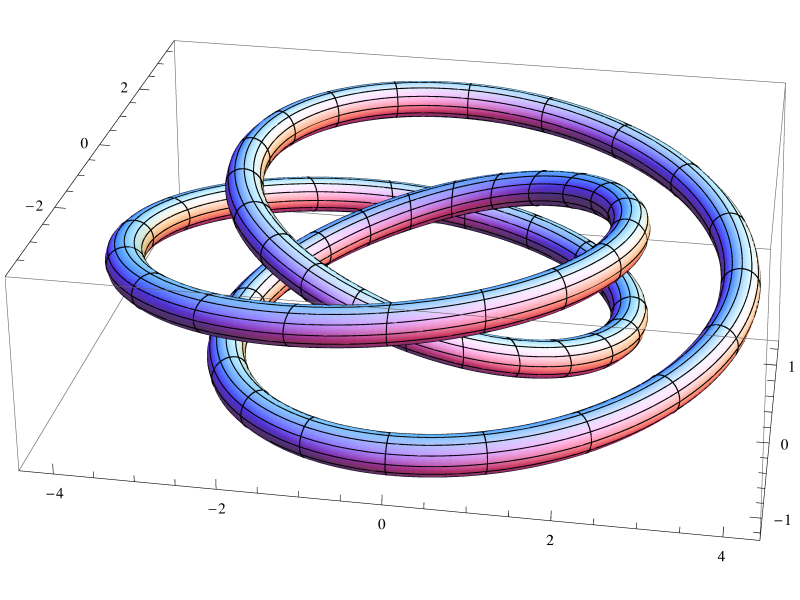
\includegraphics{KnottedTorus.png}
    }
    \caption{Verknoteter Torus}
    Quelle:  \cite{knottedtorus}
    \label{fig:knottedtorus}
\end{figure}

Dann gäbe es genau einen parallelen Schnitt durch den \cevain{cnoten}, der ein Bild wie \cref{fig:ringring} abgibt, obwohl alle \ring{ringe} und damit die Station als Ganzes ein einzelner, gewissermaßen siebenfach "`gewickelter"' Torus wäre, nämlich ein Torusknoten.

Das erklärt auch die Doppelung der Zahl $7$. Es gibt $7$ \ring{ringe} und (jeweils) $7$ \ceva{deccs}. Eine solche toroidale \ceva{cnoten}-Architektur bietet eine Erklärung für die Quasi-Identität von \ring{ringen} und \ceva{deccs}.
% Von diesen gibt es widerum verschiedene Formen, 

\paragraph{\ceva{core} als Torusknoten}

Angesichts der Bedeutung toroidaler Topologie für Fusionsreaktoren vermuten wir, dass wir hier der Topologie des \ceva{Möbius-band-accelerators} bzw. \ceva{Mino-reactors} bzw. \ceva{Cybernetischen Quecksilber-Reaktors}  auf der Spur sind (vgl.~\cref{sec:core}). \ceva{core} selber ist eine komprimierte Spiegelung der Stationsarchitektur als Ganzes. Hier entsteht durch intensive \cevain{vercnotung} die \cevain{complette verwirrung}, die für das Neuerwachen der Station nötig ist.

\paragraph{Die Raumstation als gefärbter Torusknoten}

Für jeden Torus gilt der Sieben-Farben-Satz: wie auch immer der Torus in Gebiete eingeteilt ist, es genügen genau $7$ Farben, die entstehende Landkarte einzufärben. Wir sehen hier eine topologische Begründung für die Siebenzahl der \ring{ringe}. Es könnte also eine Raumstation, deren Topologie ein (verknoteter) Torus ist, beliebig eingeteilt werden: $7$ verschiedene Kategorien von Habitaten würden genügen, um sicherzustellen, dass neben jedem Habitat ein jeweils anderes Habitat anschließt. Die Chromatische Zahl der \ceva{c-base} ist mithin ebenfalls $7$.

\begin{equation}\label{eq:chromazahl}
    \chi\left( \text{\ceva{c}}
    \right) = 7
\end{equation}

Es könnte insofern gut sein, dass $7$ \ring{ringe} eben Funktionsbereiche und nicht wirklich Kreise darstellt. 
Erschwerend kommt hinzu, dass Tori wegzusammenhängend sind; es gibt also von jedem \ring{ring} einen Weg zu jedem anderen \ring{ring}. Damit werden die wiederholten Erwähnungen von Mobilität über die \ring{ringe} hinaus bzw. zwischen ihnen plausibel.

Damit wäre die ursprüngliche Topologie ein gefärbter Torusknoten \cevain{cnoten}, mithin ein \cevain{mosaic}.

\begin{newstuff}
\lettrine{A}{n} dieser Stelle  verlassen wir  den Bereich der Empirie und begeben uns in das Reich reiner \cevain{cpeculation} bzw. purer \cevain{cience}.

Die weitere Erforschung dieser Topologie und die möglichen Ramifikationen für die energetische Effizienz des verschlungenen Miteinanders der sich ergänzenden \ring{ringe} ist eine Aufgabe ohne \cevain{endpunct}.

Uns bleibt der Hoffnung Ausdruck zu geben, dass \cevain{cünftige} Forscher die hier skizzierten Ansätze einmal zu höher Vollendung führen geworden haben werden sein können.

\ceva{vielen dank für die beachtung aller sicherheitshinweise.}
\end{newstuff}



% Und das ist ein Bild schön genug, dieses Papier zu beschließen.

% \begin{center}
%     \ceva{-- be future compatible --}    
    
%     -- be future compatible --
% \end{center}